%----------------------------------------------------------------------------------------
%	PACKAGES AND OTHER DOCUMENT CONFIGURATIONS
%------------------------------------------------------------------------
\documentclass[11pt]{article}
\usepackage[utf8]{inputenc} % Required for inputting international characters
\usepackage[T1]{fontenc} % Output font encoding for international characters
\usepackage{mathpazo} % Palatino font
\usepackage[czech]{babel} % Czech
\usepackage{graphicx}  % Graphics
%\usepackage[amsmath]

\begin{document}

%----------------------------------------------------------------------------------------
%	TITLE PAGE
%----------------------------------------------------------------------------------------

\begin{titlepage} % Suppresses displaying the page number on the title page and the subsequent page counts as page 1
	\newcommand{\HRule}{\rule{\linewidth}{0.5mm}} % Defines a new command for horizontal lines, change thickness here
	
	\center % Centre everything on the page
	
	%------------------------------------------------
	%	Headings
	%------------------------------------------------
	
	\textsc{\LARGE České vysoké učení technické v Praze}\\[1.5cm] % Main heading such as the name of your university/college
	
	\textsc{\Large Algoritmy digitální kartografie a GIS}\\[0.5cm] % Major heading such as course name
	
	\textsc{\large Katedra geomatiky}\\[0.5cm] % Minor heading such as course title
	
	%------------------------------------------------
	%	Title
	%------------------------------------------------
	
	\HRule\\[0.4cm]
	
	{\huge\bfseries Úloha č. 1: Geometrické vyhledávání bodu}\\[0.4cm] % Title of your document
	
	\HRule\\[1.5cm]
	
	%------------------------------------------------
	%	Author(s)
	%------------------------------------------------
	
	

	
	% If you don't want a supervisor, uncomment the two lines below and comment the code above
	Monika \textsc{Křížová} % Your name
	
	Marek \textsc{Hoffmann}
	
	%------------------------------------------------
	%	Date
	%------------------------------------------------
	
	\vfill\vfill\vfill % Position the date 3/4 down the remaining page
	
	{\large 18.10.2021} % Date, change the \today to a set date if you want to be precise
	
	%------------------------------------------------
	%	Logo
	%------------------------------------------------
	
	%\vfill\vfill
	%\includegraphics[width=0.2\textwidth]{placeholder.jpg}\\[1cm] % Include a department/university logo - this will require the graphicx package
	 
	%----------------------------------------------------------------------------------------
	
	\vfill % Push the date up 1/4 of the remaining page
	
\end{titlepage}

%----------------------------------------------------------------------------------------


%----------------------------------------------------------------------------------------
%	TABLE OF CONTENT
%----------------------------------------------------------------------------------------

\tableofcontents
%\thispagestyle{empty}

\clearpage

%----------------------------------------------------------------------------------------
%	ZADÁNÍ
%----------------------------------------------------------------------------------------

\section{Zadání}
Navrhněte aplikaci s grafickým rozhraním, která vyhledá a vyznačí polygon obsahující zadaný bod.

Využijte existující geografická data nebo si vytvořte vlastní soubor s nekonvexními polygony. Data načítejte z textového souboru, ve kterém jsou polygony zaznamenány ve formě špagetového modelu. 

%----------------------------------------------------------------------------------------
%	POPIS PROBLÉMU
%----------------------------------------------------------------------------------------

\section{Popis problému}
Geometrické vyhledávání bodu představuje jednu ze základních úloh digitální kartografie. 
Princip metody spočívá v určování prostorového vztahu mezi zadaným bodem $q$ a množinou $n$ bodů ${p_{i}}$ tvořících vrcholy $m$ mnohoúhelníků ${P_{j}}$ v rovině.

Úkol vyžaduje nejdříve pomocí aplikace Qt Creator vytvořit grafické prostředí aplikace a připravit si data, která jsou následně aplikací zpracována. Výstupem má být interaktivní prostředí, které zvýrazňuje polygon, v němž se nachází uživatelem zadaný bod. 


Úloha je řešena převedením problému na opakované určování polohy bodu $q$ vzhledem k mnohoúhelníku ${P_{j}}$. Pro řešení úlohy pro nekonvexní mnohoúhelníky se nejčastěji využívají algoritmy \textit {Winding Number Algorithm} a \textit{Ray Crossing Algorithm}.

%----------------------------------------------------------------------------------------
%	POPIS ALGORITMŮ
%----------------------------------------------------------------------------------------

\section{Popisy algoritmů}
\subsection{Winding Number algoritmus}
\textit {Winding Number} algoritmus je založen na výpočtu celkového úhlu $\Omega$, který musí průvodič mezi zadaným bodem $q$ a vrcholy $m$ mnohoúhelníku ${P_{j}}$ opsat nad všemi lomovými body ${p_{i}}$ polygonu. 
\begin{equation}
\Omega(q, P)=\frac{1}{2 \pi} \sum_{i=1}^{n} \omega\left(p_{i}, q, p_{i+1}\right)
\label{WN:omega_sum}
\end{equation}

Vrcholový úhel $\omega\left(p_{i}, q, p_{i+1}\right)$ se vypočte vztahem \ref{WN:omega_i}. 
\begin{equation}
\cos \omega_{i}=\frac{\vec{u}_{i} * \vec{v}_{i}}{|| \vec{u}_{i}|| * \mid \vec{v}_{i} \|} ; \vec{u}_{i}=\left(q, p_{i}\right), \vec{v}_{i}=\left(q, p_{i+1}\right)
\label{WN:omega_i}
\end{equation}

Následně se na základě vektorového součinu \ref{WN:t}
určí topologická poloha bodu a přímky procházející body $p_{i}$, $p_{i+1}$.

\begin{equation}
t=\vec{u_{i}}\times\vec{v_{i}}
\label{WN:t}
\end{equation}

Nachází-li se bod vlevo od $q$ vlevo od přímky $(p_{i}, p_{i+1})$, pak má hodnota $\omega_{i}$ kladnou hodnotu. Pokud se bod $q$ nachází vpravo od přímky $(p_{i}, p_{i+1})$, pak má hodnota $\omega_{i}$ zápornou hodnotu.\\

Pokud se rovnice (\ref{WN:omega_sum}) rovná $1$, nachází se bod $q$ v polygonu ${P_{j}}$. Pokud je výsledek nulový, pozice bodu se nachází mimo polygon ${P_{j}}$.  Uvedené vztahy popisuje rovnice (\ref{WN:omega_WN}).

\begin{equation}
\Omega(q, P)=\left\{\begin{array}{l}
1, q \in P \\
0, q \notin P \\
\end{array}\right.
\label{WN:omega_WN}
\end{equation}

\subsection{Ray Crossing algoritmus}
\textit {Ray Crossing} algoritmus je založen na docela jiném principu. 

Máme-li bod $q$ a polygon ${P_{j}}$ tvořený body ${p_{i}}$ a  vedeme-li polopřímku $r$ z bodu $q$ libovolným směrem, určuje se poloha bodu $q$ na základě počtu průsečíků $q$ polopřímky $r$ s oblastí ${P_{j}}$.

\begin{equation}
k(r, P) \% 2= \left\{\begin{array}{l}
1, q \in P \\ 
0, q \notin P \\
\end{array} \right.
\label{RC:k}
\end{equation}

V tomto tvaru je sice algoritmus rychlejší než Winding Number algoritmus, nicméně je nutné zabývat se problémem singularity, kdy bod leží na hraně polygonu či přímo inciduje s vrcholem ,nebo polopřímka $r$ prochází vrcholem ${p_{i}}$ polygonu ${P_{j}}$.

Problém singularity bude více rozebrán v následující kapitole.


%----------------------------------------------------------------------------------------
%	PROBLEMATICKÉ SITUACE
%----------------------------------------------------------------------------------------
\section{Problematické situace}

\subsection{Winding Number algoritmus}
Případ singularity u Winding Number algoritmu, kdy bod $q$ leží na hraně $h$ polygonu ${P_{j}}$ byl ošetřen následovně; Pokud se bod na hraně nachází, tak $\Omega(q, P)$ neodpovídá ani jednomu výsledku z \ref{WN:omega_WN}, tj. 

\begin{equation}
\Omega(q, P) \neq 1 \wedge \Omega(q, P) \neq 0, \quad q \in h
\end{equation}


\subsection{Ray Crossing algoritmus}
Prochází-li polopřímka $r$ jedním z vrcholů ${p_{i}}$ polygonu ${P_{j}}$ či jeho hranou $h$, dochází k tzv. singularitě.

Pro odstranění této singularity se zavádí varianta Ray Crossing algoritmu s redukcí ke $q$. V této metodě se vytváří lokální souřadnicový systém $(q,x',y')$ s posunutím bodů ${p_{i}}$ o hodnotu $q$. 

Lokální souřadnicová soustava je popsána následovně:
\begin{itemize}
\item Počátek v bodě q
\item osa $x^{\prime}$ rovnoběžná s osou x
\item osa $y^{\prime}$ rovnoběžná s osou y
\end{itemize}

Redukce popisují následující rovnice.

\begin{eqnarray}
x_{i}^{\prime}=x_{i}-x_{q}\, \nonumber \\
y_{i}^{\prime}=y_{i}-y_{q} \
\end{eqnarray}
\begin{eqnarray}
x_{i-1}^{\prime}=x_{i-1}-x_{q}\, \nonumber \\
y_{i-1}^{\prime}=y_{i-1}-y_{q} \,
\end{eqnarray}

Zdali existuje průsečík přímky $p$ a paprsku $r$ zjistíme následující podmínkou

\begin{equation}
\left(y_{i}^{\prime}>0\right) \wedge\left(y_{i-1}^{\prime}<=0\right) \vee\left(y_{i-1}^{\prime}>0\right) \wedge\left(y_{i}^{\prime}<=0\right)
\end{equation}

Pokud existuje, vypočítáme jeho x-ovou souřadnici podle \ref{RC:xm}.

\begin{equation}
x_{m}^{\prime}=\frac{x_{i}^{\prime} y_{i-1}^{\prime}-x_{i-1}^{\prime} y_{i}^{\prime}}{y_{i}^{\prime}-y_{i-1}^{\prime}}
\label{RC:xm} 
\end{equation}

Následně pak hledáme pouze ty průsečíky $M$, které se nachází v pravé polorovině $\sigma_{r}$.

\begin{equation}
k(r, P)=\left\{\begin{array}{l}
k(r, P)+1, x_{m}^{\prime}>0 \\ 
k(r, P), x_{m}^{\prime} <= 0
\end{array}\right.
\end{equation}

Zda bod leží v polygonu zjistíme dle rovnice rovnice \ref{RC:k}.

Případ singulárního případu, kdy bod leží na hraně polygonu nebyl v naší aplikaci ošetřen.

\clearpage



%----------------------------------------------------------------------------------------
%	VSTUPNÍ DATA
%----------------------------------------------------------------------------------------


\section{Vstupní data}

Polygonová mapa se do projektu nahrává z textového souboru, který musí splňovat specifický formát, bez něhož nebude zajištěno správné načítání dat.  

Vrcholy polygonů jsou načítány postupně řádek po řádku, přičemž musí v nahrávaném souboru platit následující pravidla:    

\begin{itemize}
\item každý vrchol polygonu je definován na jednotlivém řádku,
\item na řádku je pořadí proměnných id >> x >> y   ,  hodnoty jsou od sebe odděleny  jednou mezerou,
\item id je identifikátor jednotlivých vrcholů polygonu, x a y jsou souřadnice vrcholů polygonu,    
\item nový polygon má vždy hodnotu id prvního vrcholu rovnu 1, od této hodnoty  se  postupně načítají body, a  to až do okamžiku,  kdy program dojde  k dalšímu identifikátoru s označením 1.   
\end{itemize}

\begin{figure}[htbh]
	\centering
	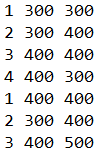
\includegraphics[scale=1]{images/vstup.png} 
	\caption{Špagetový model vstupního souboru}
	\label{fig:vstup.}
\end{figure} 

Souřadnice bodu $q$ jsou získávány interaktivně odečtením souřadnic kurzoru myši.   

%----------------------------------------------------------------------------------------
%	VÝSTUPNÍ DATA
%----------------------------------------------------------------------------------------

\section{Výstupní data}

Po načtení souboru s polygonovou mapou, přidání bodu $q$ a stisknutí tlačítka Analyze se v místě vyznačeném na obrázku \ref{fig:app_analyze} vytiskne výsledek analýzy polohy bodu. 

\begin{figure}[htbh]
	\centering
	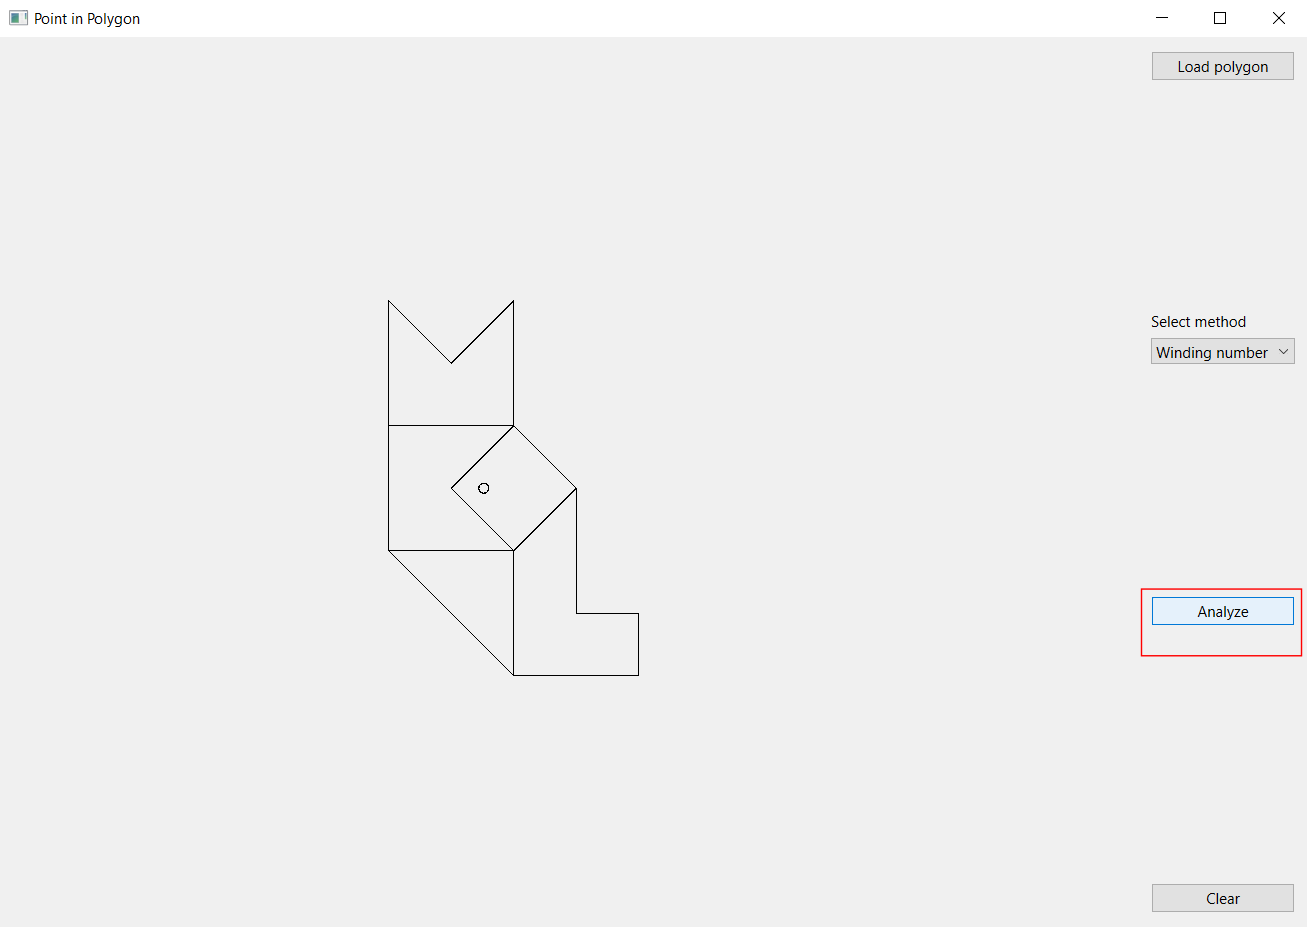
\includegraphics[scale=0.4]{images/aplikace_klik_analyze.png} 
	\caption{Aplikace s načteným polygonem}
	\label{fig:app_analyze}
\end{figure} 

Výsledek dotazu může mít 3 různé hodnoty:

\begin{itemize}
\item je-li bod mimo polygonovou mapu, vypíše se zpráva „Outside“,
\item je-li bod uvnitř polygonu, vypíše se zpráva „Inside“ a polygon obsahující zadaný bod se graficky zvýrazní,
\item je-li bod na hranici polygonu, vypíše se „Point is on the line“ a graficky se zvýrazní polygon, na jehož linii bod leží.      
\end{itemize}
\begin{figure}[htbh]
	\centering
	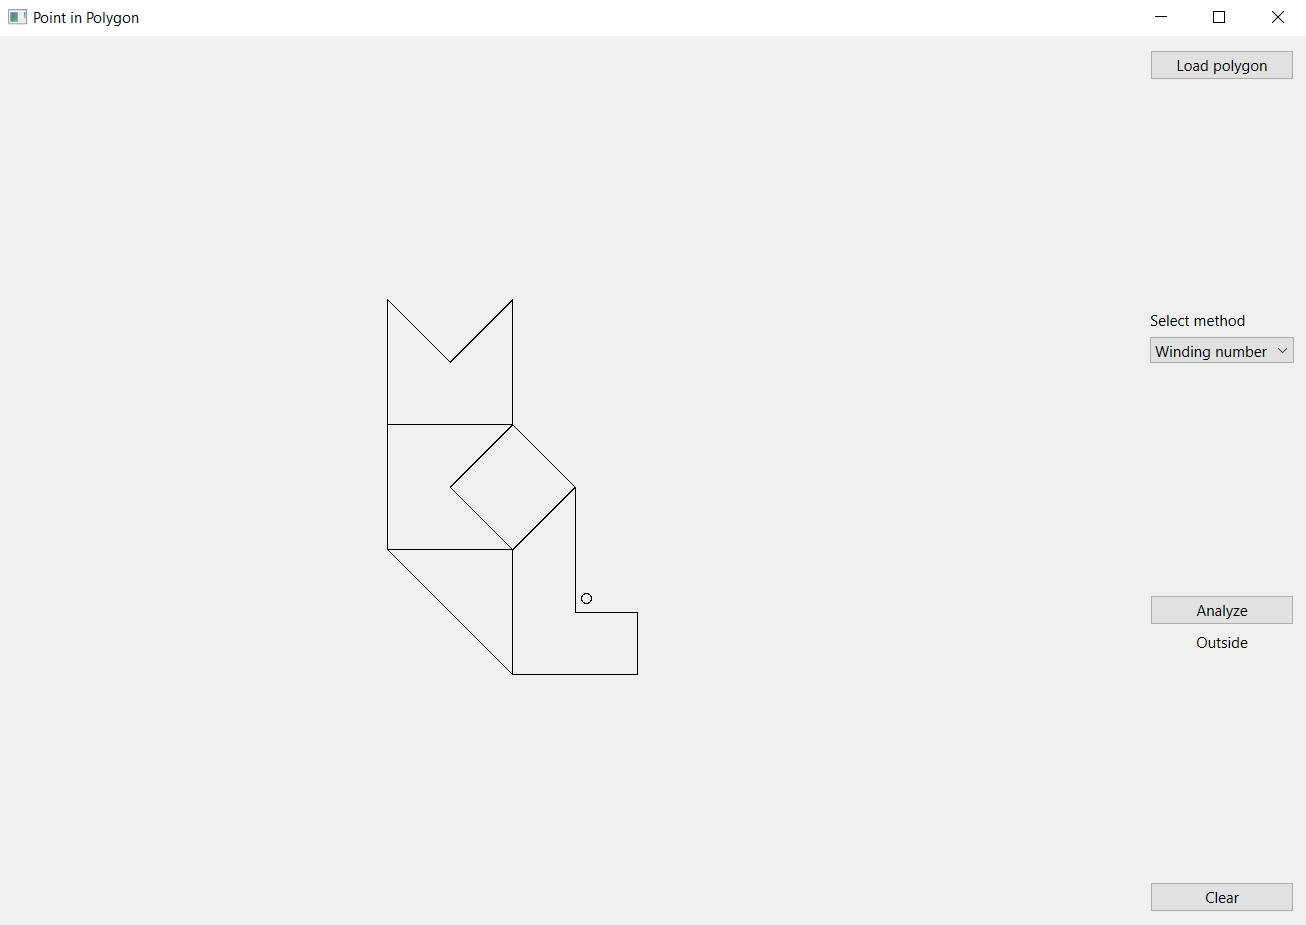
\includegraphics[scale=0.4]{images/aplikace_analyze_outside.png} 
	\caption{Bod vně polygonu}
	\label{fig:app_outside}
\end{figure} 
\begin{figure}[htbh]
	\centering
	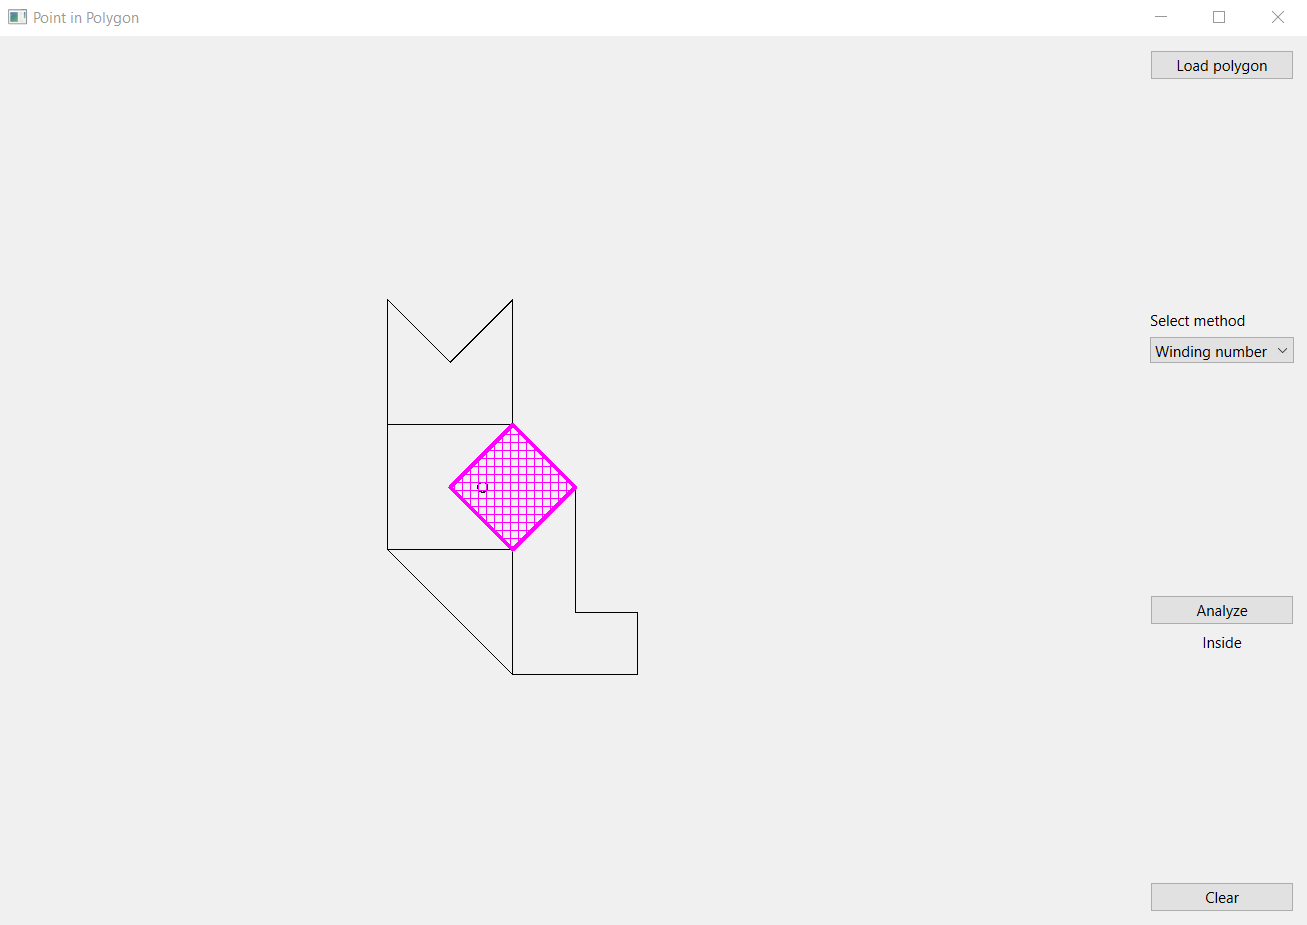
\includegraphics[scale=0.4]{images/aplikace_analyze_inside.png} 
	\caption{Bod uvnitř polygonu}
	\label{fig:app_inside}
\end{figure} 


\clearpage

\section{Printscreen vytvořené aplikace}
\begin{figure}[htbh]
	\centering
	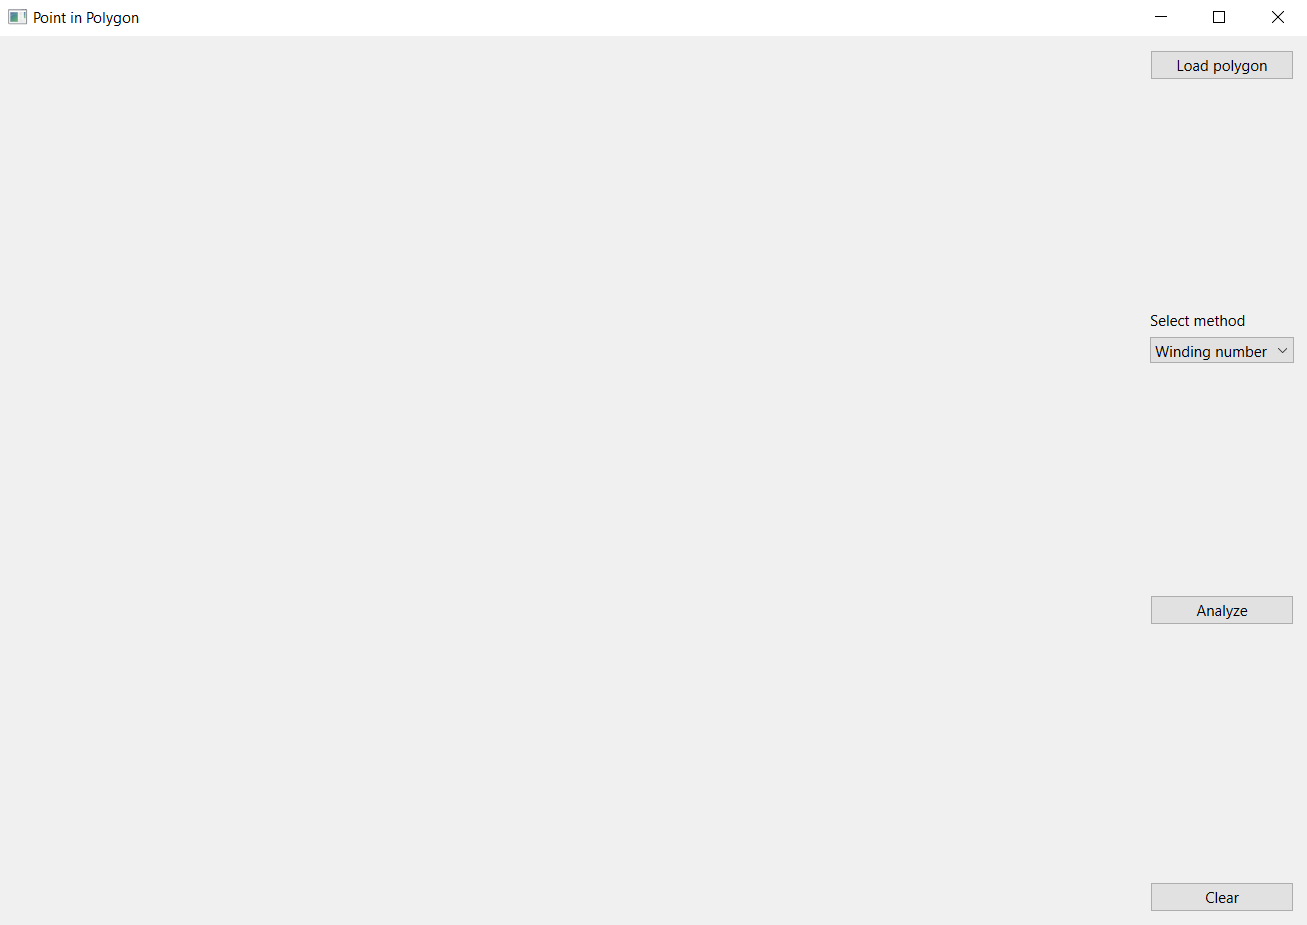
\includegraphics[scale=0.4]{images/aplikace_uvodni_okno.png} 
	\caption{Úvodní okno aplikace}
	\label{fig:uvodni_okno}
\end{figure} 

%----------------------------------------------------------------------------------------
%	DOKUMENTACE
%----------------------------------------------------------------------------------------

\section{Dokumentace}
Kód zahrnuje 3 třídy – Draw, Algorithms a Widget, které budou následně detailněji popsány.      

\subsection{Třída Algorithms}
Třída Algorithms obsahuje 4 funkce :  

\begin{itemize}
\item int getPointLinePosition(QPoint \&a, QPoint \&p1, QPoint \&p2);
\item double get2LinesAngle(QPoint \&p1, QPoint \&p2, QPoint \&p3, QPoint \&p4);
\item int getPositionWinding(QPoint \&q, std::vector<QPoint> \&pol);
\item int getPositionRayCrossing(QPoint \&q, std::vector<QPoint> \&pol);
\end{itemize}

\paragraph{int getPointLinePosition(QPoint \&a, QPoint \&p1, QPoint \&p2);}\mbox{}\\
Analyzuje vzájemnou polohu mezi bodem a linií polygonu, resp. v jaké polorovině vůči linii se bod nachází. Vstupními argumenty funkce jsou souřadnice určovaného bodu (jako QPoint) a souřadnice 2 bodů určujících polohu linie (vrcholy polygonu taktéž jako QPoint). Funkce vrací vždy buď hodnotu 1, 0 nebo -1 dle následujících pravidel:

\begin{itemize}
\item 0 v případě, že bod leží v pravé polorovině,
\item 1 v případě, že  bod leží v levé polorovině,
\item -1 v případě, že bod leží na linii.
\end{itemize}

\paragraph{double get2LinesAngle(QPoint \&p1, QPoint \&p2, QPoint \&p3, QPoint \&p4);}\mbox{}\\
Počítá úhel mezi dvěma liniemi pomocí vztahu \ref{WN:omega_i}, vstupními argumenty jsou body určující linie -  tedy vrcholy polygonu). Návratovou hodnotou funkce je double – desetinné číslo s velikostí úhlu mezi těmito přímkami.  

\paragraph{int getPositionWinding(QPoint \&q, std::vector<QPoint> \&pol);}\mbox{}\\
Funkce analyzuje polohu bodu metodou Winding number, jež byla podrobně vysvětlena v kapitole 3.  Vstupními argumenty jsou souřadnice bodu Q (jako QPoint) a vektor vrcholů polygonu (vektor naplněný prvky QPoint). Funkce vrací integer, jež může nabývat 3 hodnot:

\begin{itemize}
\item 1, leží-li analyzovaný bod uvnitř polygonu
\item -1 leží-li na linii polygonu 
\item a 0, leží-li mimo kontrolovaný polygon.
\end{itemize}

\paragraph{int getPositionRayCrossing(QPoint \&q, std::vector<QPoint> \&pol);}\mbox{}\\
Funkce analyzuje polohu bodu metodou Ray Crossing, jež byla podrobně vysvětlena v kapitole 3. vstupními argumenty jsou souřadnice bodu Q (jako QPoint) a vektor vrcholů polygonu (vektor naplněný prvky QPoint). Funkce vrací, stejně jako funkce předchozí, celé číslo, jež může nabývat následujících hodnot:

\begin{itemize}
\item 1, pokud leží analyzovaný bod uvnitř polygonu
\item a 0, leží-li mimo kontrolovaný polygon.
\end{itemize}

Ošetření případu, kdy bod leží na linii nebylo do kódu implementováno, funkce tedy nevrací  hodnotu -1, leží-li bod na linii.

\subsection{Třída Draw}
Třída Draw obsahuje následující funkce, které budou dále podrobně popsány:

\begin{itemize}
\item void paintEvent(QPaintEvent *event);
\item void mousePressEvent(QMouseEvent *event);
\item void clear();
\item QPoint getPoint(){return q;}
\item std::vector<QPolygon> getPolygon()\{return polygons;\}
\item void fillPolygon(int result);
\item void loadData(QString \&file\_name);
\end{itemize}

a následující proměnné:

\begin{itemize}
\item std::vector<QPolygon> polygons;  
\item QPoint q; - analyzovaný bod
\item int highlighted\_polygon=-99; - id polygonu, který obsahuje analyzovaný bod   
\end{itemize}

\paragraph{•	void paintEvent(QPaintEvent *event);}\mbox{}\\
Funkce nastavuje grafické atributy vykreslovaných objektů a kreslí na plátno vyhodnocovaný bod a zadané polygony a znázorňuje polygon incidující s bodem. 

\paragraph{void mousePressEvent(QMouseEvent *event);}\mbox{}\\
Metoda získává souřadnice myši a ukládá je do proměnné QPoint q, tedy jako souřadnice analyzovaného bodu Q.

\paragraph{void clear();}\mbox{}\\
Funkce smaže veškeré objekty, jež jsou vykresleny na canvasu, funkce nemá vstupní argumenty. 

\paragraph{QPoint getPoint()\{return q;\}}\mbox{}\\
Funkce vrací souřadnice bodu Q, návratový typ funkce je QPoint, funkce nemá vstupní argumenty.

\paragraph{std::vector<QPolygon> getPolygon()\{return polygons;\}}\mbox{}\\
Funkce vrací vektor polygonů načtených z textového souboru – návratový typ je std::vector<QPolygon>, funkce nemá vstupní argumenty.

\paragraph{void fillPolygon(int result);}\mbox{}\\
Funkce ukládá identifikátor polygonu obsahujícího analyzovaný bod, pomocí identifikátoru se tento polygon následně ve funkci paintEvent() zvýrazní. Vstupním argumentem je int result, jež stanovuje polohu bodu vůči linii (má hodnoty 0,1,-1,dle definice výše). 

\paragraph{void loadData(QString \&file\_name);}\mbox{}\\
Funkce načítá data z textového souboru a ukládá je do vektoru QPolygon. Vstupní argumentem je cesta k souboru, jež chceme načíst do aplikace.   

\subsection{Třída Widget}
Třída Widget obsahuje 3 metody:

\begin{itemize}
\item void on\_pushButtonClear\_clicked();
\item void on\_pushButtonAnalyze\_clicked();
\item void on\_pushButtonLoad\_clicked();
\end{itemize}

\paragraph{ void on\_pushButtonClear\_clicked();}\mbox{}\\
Funkce se volá při stisknutí tlačítka Clear, volá funkci clear(), jež je definovaná v třídě Draw.

\paragraph{ void on\_pushButtonAnalyze\_clicked();}\mbox{}\\
Funkce se volá při stisknutí tlačítka Analyze. Ve funkci nejprve dojde k uložení jednotlivých polygonů do vektoru vrcholů polygonu, následně je zavolána funkce getPositionRayCrossing ze třídy Algorithms nebo getPositionWinding dle výběru v comboboxu.

\paragraph{void on\_pushButtonLoad\_clicked();}\mbox{}\\
Funkce slouží k inicializaci načítání souboru, spustí se po stisknutí tlačítka Load, čímž zobrazí dialog pro výběr souboru obsahujícího data, jež mají být načtena do aplikace. Po výběru souboru se zavolá funkce loadData ze třídy Draw, která přečte data ze souboru a uloží je do proměnné.

%----------------------------------------------------------------------------------------
%	ZÁVĚR
%----------------------------------------------------------------------------------------

\section{Závěr}
Vytvořená aplikace vizualizuje polygonovou mapu uloženou ve výše popsaném formátu, po přidání bodu taktéž analyzuje polohu tohoto bodu vůči jednotlivým polygonům mapy. Po analýze bodu se vypíše výsledek – tedy zda bod leží uvnitř nebo vně polygonové mapy, v případě umístění bodu uvnitř polygonu se polygon obsahující tento bod graficky zvýrazní.\\

 V aplikaci jsou pro vyhodnocení polohy bodu implementovány 2 algoritmy – Winding number a Ray Crossing, mezi nimiž je možné přepínat pomocí comboboxu umístěném v pravé části okna. Princip fungování obou algoritmů je popsán v kapitole 3. \\

Možné zlepšení kódu programu by bylo v řešení singularit polohy bodu $q$, tedy případu, kdy bod $q$ leží na vrcholu jednoho či více polygonů a dále přidání analýzy případu, kdy bod $q$ leží na linii polygonu pomocí Ray Crossing algoritmu. Dalším možným krokem pro zlepšení funkčnosti by mohlo být přidání bodu $q$ pomocí vepsání souřadnic, nikoliv pouze odečtením polohy myši.

\end{document}
